\chapter{Haskell}
\label{sec:Haskell}
\section{Allgemein}
Haskell ist eine Funktionale Programmiersprache und ist daher um einiges anders als die bisher gelernten Objektorientierten Sprachen. Diese verwenden verstärkt funktionale Eigenschaften um sich weiter zu entwickeln. Funktionale Sprachen sind frei von Seiteneffekten und die Methoden können sich Gegenseitig nicht beeinflussen. Eine Methode liefert bei den gleichem Input immer den gleichen Output.
In diesem Dokument werden verstärkt Codebeispiele genutzt um die Sprache kurz zu erläutern. 
\section{Input, Main, Output}
Zunächst ein kleines "Hello World" Beispiel, wie es zu jeder Sprache gehört. Hier sieht man direkt wie die main von Haskell aufgebaut ist.
\newline
\begin{lstlisting}[language=Haskell]  
main = putStrLn "Hello World"
\end{lstlisting}
\qquad\newline
Um ein kleines Programm zu schreiben, was mehr tut, als lediglich Sachen auszugeben, müssen wir Input verarbeiten. Dafür ist Haskell nie wirklich vorgesehen worden, da dies unvorhergesehenes Verhalten erzeugen kann, welche Haskell vermeiden soll. Daher sollte man dies nur verwenden, wenn es gefordert oder nicht anders möglich ist. 
\newline
\begin{lstlisting}[language=Haskell]  
main = 	do
	print "What is your name?"
	name <- getLine
	print("Hello" ++ name ++ "!")
	-- main 
\end{lstlisting}
\qquad\newline
Wie man sieht, kann man den Input in eine vorher nicht definierte variable geben. In Haskell muss man variablen nicht vorher genauer definieren. Der Compiler versucht zur Compilezeit zu ermitteln, welchen Typ die Variable hat und setzt diesen fest. Wenn dies nicht möglich ist, wird die Variable zur Laufzeit erstellt und definiert und genau das kann zu unvorhergesehenem Verhalten führen. 
\subsection{IO}
IO Programme aus der Fragestunde, härter als das wird es aller Voraussicht nach nicht werden. 
\begin{lstlisting}[language=Haskell]  
putToConsoleAndCheck :: String -> IO Bool
putToConsoleAndCheck s = do
	if s == "" then return False 
	else do
	putStrLn s
	return True


putToConsoleAndReturnNothing :: String -> IO ()
putToConsoleAndReturnNothing s = do
	if s == "" then return () 
	else do
	putStrLn s
	return ()
\end{lstlisting}
\section{Funktionsdeklaration}
Eine Funktion in Haskell sieht ungewohnt aus und erinnert mich immer stark an Mathe. Wobei die späteren Listen Verarbeitungsmöglichkeiten noch stärker an die Mathematik angelehnt sind.
\newline
\begin{lstlisting}[language=Haskell]  
f :: Int -> Int -> Int
f x y = x*x + y*y
\end{lstlisting}
\qquad\newline
dies ist alles was genötigt wird um eine Funktion zu deklarieren. Vom Schreibaufwand ist dies sehr gering. Jedoch ist es ungewohnt eine Funktion so zu sehen. Also nehmen wir diese einmal komplett auseinander. 
\qquad\newline\qquad\newline
$\overbrace{f}^\text{Funktionsname} \underbrace{x \quad y}_\text{Variablennamen der Funktion} = \overbrace{x*x+y*y}^\text{was die Funktion macht}$
\qquad\newline\qquad\newline

Es sieht zwar nicht gerade überragend aus, jedoch ist hier schon sehr genau erklärt wie eine Funktion aufgebaut ist. 
$f :: Int -> Int -> Int$ ist die sogenannte Funktionstypendeklaration das erste $Int$ steht für das $x$ das zweite für $y$ und das dritte für den Typ des Ergebnisses. Es ist zwar nicht notwendig dies anzugeben, jedoch fördert es das Verständnis und hilft einem dabei nochmals genau über die Funktion nachzudenken. Da diese Methode jedoch auch gut für alle Zahlen geeignet ist, sollte man den Funktionstypen umdefinieren
\newline
\begin{lstlisting}[language=Haskell]  
f :: Num a => a -> a -> a 
\end{lstlisting}
\qquad\newline
Das sind nochmals kryptischer aus, jedoch bedeutet dies nur, dass die Funktion $f$ eine Zahl ($Num a =>"$) vom Typ $Num$ erwartet. Danach hätte es gerne noch eine Zahl und gibt eine Zahl zurück. Welche Typen diese Zahlen haben, wird zur Compilezeit definiert und entsprechend angewandt. Das $a->a->a$ bedeutet, dass alle vom Typ $Num$ sein müssen. Also wenn wir als erstes ein Int eingeben, werden alle $a$ zu einem Int und es werden nur noch Int's erwartet. Vorteil, wir können eine Funktion für unterschiedliche Zahlentypen verwenden, ohne diese jedes mal neu zu definieren. 

Auch können Funktionen weitere Funktionen aufrufen.
\newline
\begin{lstlisting}[language=Haskell]  
f :: Num a => a -> a -> a 
f x y = x*x + y*y

g :: Num a => a -> a -> a 
g = f 3
\end{lstlisting}
\qquad\newline

Wi funktioniert nun $g$? diese Funktion ruft nun $f$ mit dem Wert 3 auf und $f$ gibt sich die Funktion $f$ zurück um noch einen Wert entgegen zu nehmen. Dies bezeichnet man auch als Currying. 
Um zu verhindern, dass Haskell weiterhin die Typ Transformationen von Variablen übernimmt, kann man diese vorher definieren. Davon wird abgeraten, da dies zu unvorhergesehen Fehlern führen kann. z.B. wird der nach führende Code nie erfolgreich ausgeführt werden. 
\newline
\begin{lstlisting}[language=Haskell]  
x:: Int
x = 3

y:: Float
y=2,4

print (f x)
\end{lstlisting}
\qquad\newline

\section{Notation}
\subsection{Logik}

\begin{tabular}{cccc}
|| $\Rightarrow$ or 	& \&\& $\Rightarrow$ and  & ==  $\Rightarrow$ Gleichheit & /= $\Rightarrow$ Differenz  \\ 
\end{tabular} 

\subsection{Potenz}
\begin{tabular}{cc}
 x\^{}n & x**y \\  
\end{tabular} 

Hierbei gilt es zu beachten, dass n ein Int || Integer sein muss, und y irgend eine Variable vom Typ Num sein darf. 

\subsection{Listen}

\begin{itemize}
	\item sind getypt, es können lediglich Elemente eines Typs in einer Liste vorkommen (Mischen von Typen ist nicht möglich). Dies ergänzt sich mit Tupeln: Listen sind theoretisch beliebig lange Folgen von Elementen eines Typs, Tupel sind definiert lange Folgen von Elementen, die verschiedene Typen haben können. Typsignatur von Listen: z.B. [Int], [Char], usw.
	\item können polymorph sein, d.h., der Typ einer Liste kann parametrisiert werden. Typsignatur in diesem Fall: z.B. [a]
	\item können per Aufzählung der Elemente definiert werden (Beispiel: [1,2,3]) oder mittels des Listenkonstruktors (Beispiel: 1:(2:(3)) ).
	\item werden per Rekursion (x:xs beschreibt das erste Element x einer Liste und die Restliste xs) oder per Indizierung (Operator !!) verarbeitet (die Indizierung beginnt bei 0)
	\item können mittels Erzeugungsschemata beschrieben werden (list comprehensions): z.B. [ transform neueListe | neueListe <- alteListe, tollerTest neueListe ], in dem die Elemente einer existierenden Liste traversiert, optional mit Prädikaten gefiltert und ebenfalls optional durch weitere Funktionen transformiert in eine neue Liste übernommen werden. In diese Rubrik fällt auch eine abgekürzte Schreibweise für Aufzählungen: z.B. [1..10] um eine Liste mit Elementen von 1 bis 10 zu erzeugen.
	\item können dank Haskell´s Lazy Evaluation Strategie unendlich lang sein (ihrer Beschreibung nach), wie z.B. bei [1..]. Solche Listen können verwendet werden, solange für den gewünschten Zweck die Auswertung nur eines Teils der Liste ausreicht.
\end{itemize}

\subsubsection{Beispiele}
\begin{align*}
\text{[ ]} &\Leftrightarrow \text{leere Liste}\\
\text{[1,2,3]} &\Leftrightarrow \text{Liste von integralen}\\
\text{["foo","bar","baz"]} &\Leftrightarrow \text{Liste aus Strings}\\
\text{1:[2,3]} &\Leftrightarrow \text{[1,2,3] : ist das Symbol zum vorne anhängen an eine Liste}\\
\text{1:2:[ ]} &\Leftrightarrow \text{[1,2]}\\
\text{[1,2]++[3,4]} &\Leftrightarrow \text{[1,2,3,4] ++ ist für das konkatinieren zuständig}\\
\text{[1,2,3]++["foo"]} &\Leftrightarrow \text{Error, die Inahlte einer Liste müssen immer vom selben Typ sein.}\\
\text{[1..4]} &\Leftrightarrow \text{[1,2,3,4]}\\
\text{[1,3, .. 10]} &\Leftrightarrow \text{[1,3,5,7,9]}\\
\text{[2,3,5,7,11 ... 100]} &\Leftrightarrow \text{Haskell ist leider nicht so klug ;-) }\\
\text{[10,9 ..1]} &\Leftrightarrow \text{[10,9,8,7,6,5,4,3,2,1]}\\
\end{align*}

\subsection{Strings $\Rightarrow$ Liste aus Char}
'a' :: Char\\
\grqq  a\grqq   :: [Char]\\
\grqq  \grqq   $\Leftrightarrow$ []\\
\grqq  ab\grqq   $\Leftrightarrow$  ['a','b'] $\Leftrightarrow$  'a':\grqq  b\grqq   $\Leftrightarrow$ 'a':['b'] $\Leftrightarrow$  'a':'b':[]\\
\grqq  abc\grqq   $\Leftrightarrow$  \grqq  ab\grqq   ++ \grqq  c\grqq  

\subsection{Tupel}
Tupel können unterschiedliche Typen enthalten und beliebig groß sein, jedoch funktionieren die Standard Implementationen lediglich auf Tupel der Größe 2\\
\subsection{Beispiele}
\subsubsection{Tupelkonstruktionen}
(2,\grqq foo\grqq  ) Unterschiedliche Typen sind legitim in Tupel\\
(3,'a',[2,3]) Listen sind auch möglich in Tupel\\
((2,\grqq a\grqq),\grqq c\grqq ,3) Auch können Tupel in Tupel geschrieben werden\\
\subsubsection{Standardimplementationen}
fst(x,y) $\Rightarrow$ x \\
fst(x,y,z) $\Rightarrow$ Error, zu viele Elemente \\
snd(x,y) $\Rightarrow$ y\\
snd(x,y,z) $\Rightarrow$ Error, zu viele Elemente

\section{Currying}
Grundsätzlich sind alle Funktionen in Haskell curried. Curried bedeutet, dass die Funktion eine Funktion zurück liefert welche eine weitere Variable erwartet. 
\newline
\begin{lstlisting}[language=Haskell]  
f :: Num a => a -> a -> a 
f x  = x*x + y*y
\end{lstlisting}
\qquad\newline
Bei diesem Beispiel wird die Funktion mit $f$ 4 5 aufgerufen. Als erstes Ergebnis liefert die Funktion sich selbst zurück und nimmt die 5 als $y$ auf. Dadurch ist es möglich Funktionen kürzer zu gestalten. In den folgenden Beispielen als erstes die gecurriede Version und direkt im Anschluss die nicht gercurriede Version. 
\newline
\begin{lstlisting}[language=Haskell]  
Klassisches Currying
sum x y = x + y

Klassische ugecurriede Version
sum (x,y) = x + y
\end{lstlisting}
\qquad\newline
Auch lassen sich die Funktionen einfach Verkürzen. 
\begin{lstlisting}[language=Haskell]  
Ungecurriede Version
square :: Num a => a -> a
square x = x^2

Gecurriede Version
square :: Num a => a -> a
square' = (^2)
\end{lstlisting}
\section{if .. then .. else und Guards}
Hier einfach ein Beispiel der gleichen Funktion einmal mit if .. then .. else Konstrukt und einmal als Guards (diese erinnern mich immer sehr stark an Switches) welche auch mit Pattern Matching zusammenarbeiten. Bei einem if .. then .. else Konstrukt muss immer ein else Teil angegeben werden. Da der Compiler sonst streikt. Denn Funktionen sollen ohne Nebeneffekte ausgeführt werden können. Und ein Vergessenes else führt zu nicht vorhersagbaren Nebeneffekten. 
\begin{lstlisting}[language=Haskell]  
absolute :: (Ord a, Num a) => a -> a
absolute x = if x >= 0 then x else -x

absolute' :: (Ord a, Num a) => a -> a
absolute' x 
	| x >= 0 =x
	| otherwise = -x
\end{lstlisting}
\qquad\newline

\section{Typen und Typ Klassen}
\subsection{Standard Typen}
\qquad\\
\textbf{Int} ist ein ganzzahliger, an das System gebundener Wert. 32-Bit / 64-Bit\\ 
\textbf{Integer} ist auch ein ganzzahliger, nicht an das System gebundener Wert, es kann so groß werden, wie der Speicher groß ist. \\
\textbf{Float} eine echte Gleitkommazahl mit einfacher Genauigkeit. \\
\textbf{Double} eine echte Gleitkommazahl mit doppelter Genauigkeit. \\
\textbf{Bool} Boolean halt. \\
\textbf{Char} ein einzelnes Zeichen in Einfachen Anführungszeichen. 
\subsection{Standard Typ Klassen}\qquad\\
\textbf{Eq} 
\begin{lstlisting}[language=Haskell]  
(==) :: (Eq a) => a -> a -> Bool  
\end{lstlisting}\qquad\newline
\textbf{Ord} 
\begin{lstlisting}[language=Haskell]  
(>) :: (Ord a) => a -> a -> Bool  
\end{lstlisting}\qquad\newline
\textbf{Show} wandelt Zahlen und boolische Ausdrücke in Strings um\
\begin{lstlisting}[language=Haskell]  
show :: Show a => a -> String 
\end{lstlisting}\qquad\newline
\textbf{Read} wandelt Strings in Zahlen oder boolische Ausdrücke um. 
\begin{lstlisting}[language=Haskell]  
read :: (Read a) => String -> a  
\end{lstlisting}\qquad\newline
\textbf{Num} ist eine numerische Typ Klasse. Ihr Mitglieder lasen sich wie Zahlen benutzen und verhalten sich so.\\
\textbf{Enum} ist eine Typ Klasse, welche alle auf zählbaren / durchzunummerierende Sachen enthalten. dadurch lassen sich erst die unendlichen Listen darstellen. Auch können succ und pred als Funktionen auf dessen Mitglieder angewandt werden.  

\subsection{Eigene Typklassen}\qquad\\
\textbf{type Name = AnotherType}\\ Damit kann man dem Kind AnotherType einen neuen Namen geben. Wenn man z.B. zwischen Nachname und Vorname unterscheiden möchte. Jedoch macht der Compiler hier keinen Unterschied. \\\qquad\\
\textbf{data Name = NameConstructor AnotherType}\\ Hier macht der Compiler eine Unterscheidung. Der genaue Unterschied zwischen beiden type und data wird gleich an einem Beispiel erläutert.  \\\qquad\\
\textbf{data} \\ Damit kann man sich rekursive Strukturen definieren.\\\qquad\\
\textbf{deriving}\\ damit kann man sich Funktionen erzeugen lassen. 

\subsubsection{Beispiele}
Bei dem nachfolgenden Beispiel, muss man sehr aufpassen, denn die Type und Data Version haben starke Unterschiede zur Laufzeit. Wenn man die Type Version nutzt, kann man als Eingabe Color und Name vertauschen und das Programm arbeitet trotzdem weiter, da es lediglich Strings erwartet. \\
Bei Data erwartet Haskell wirklich Datenstrukturen Name und Color. Wenn man hier zuerst Color und danach Name eingibt, meckert der Compiler. 

\begin{lstlisting}[language=Haskell]  
Type Version
type Name   = String
type Color  = String

Data Version
data Name   = NameConstr String
data Color  = ColorConstr String

showInfos :: Name ->  Color -> String
showInfos (NameConstr name) (ColorConstr color) =
"Name: " ++ name ++ ", Color: " ++ color
\end{lstlisting}\qquad\newline
Als nächstes wird eine Rekursive Datenstruktur definiert und mit deriving(Show) erweitert, was dazu führt, das diese Datenstruktur direkt gedruckt werden kann. 
\begin{lstlisting}[language=Haskell]  
data Tree a = EmptyTree | Node a (Tree a) (Tree a) deriving (Show, Read, Eq)  
\end{lstlisting}
\section{Pattern Matching}\label{sec:hpm}\qquad\\
Beim Pattern Matching handelt es sich um die Möglichkeit in eine Funktion Abzweigungen einzubauen, aufgrund von bestimmten Inhalten einer Variable. Davon wird exzessiv in Prolog$^{\ref{sec:Prolog}}$ gebraucht gemacht. \\
Das Pattern Matching ist eine effiziente Art zu programmieren, wenn man wenige unterschiedliche Werte hat, auf die geprüft werden muss. Auch kann man damit gut Abbruchbedingungen erstellen für rekursive Funktionen. Dabei gilt zu beachten, dass von oben nach unten gearbeitet wird. 
\begin{lstlisting}[language=Haskell]
factorial :: (Integral a) => a -> a  
factorial 0 = 1  
factorial n = n * factorial (n - 1)  
\end{lstlisting}
\section{List Comprehension}
Mit List Comprehensions kann man einfach Listen nach zuvor definierten Regeln erstellen. Dies ist besonders nützlich, um viele Werte schnell zu generieren.
\subsection{Beispiele}
\begin{lstlisting}[language=Haskell]
[x^2|x<-[1..5]]
Ergebnis: [1,4,9,16,25] 
\end{lstlisting}
Der Bereich nach | ist der sogenannte Generatorbereich und wird dazu genutzt, die Regeln für das erstellen der einzelnen Variablen zu definieren. \\ 
\begin{lstlisting}[language=Haskell]
[(x,y)|x <- [1,2,3],y <- [4,5]]
Ergebnis: [(1,4),(1,5),(2,4),(2,5),(3,4),(3,5)] 
\end{lstlisting}
Man kann auch mehrere Variablen im Generator Bereich verwenden und dadurch eine Liste von Tupeln generieren wie im oberen Beispiel gezeigt.  Jedoch sollte man sehr auf die Reihenfolge der Generatoren achten, da diese das Ergebnis stark beeinflussen. \\
\begin{lstlisting}[language=Haskell]
[(x,y)|x <- [1,2,3],y <- [x..3]]
Ergebnis: [(1,1),(1,2),(1,3),(2,2),(2,3),(3,3)] 
\end{lstlisting}
Hier werden Dependant Generators verwendet. Die zu erzeugenden Werte für $y$ hängen von $x$ ab. Dadurch kann man sehr gut doppelte Werte vermeiden und andere Spielereien machen. \\

\section{Lambda ( $\lambda$ ) Funktionen}\qquad\\
Lambda Funktionen sind Namenlose Funktionen welche lediglich einmal verwendet werden. Dies macht es möglich Funktionen in Methoden zu definieren und hat unter anderem auch Einzug in Java gefunden. Lambda Funktionen werden mit einem $\backslash$ eingeleitet. Hier ein Beispiel für eine einfache Addition.\\
\begin{lstlisting}[language=Haskell]
(\x y -> x+y) 4 3
Ergebnis: 7
\end{lstlisting}\qquad\\
Auf diese Art und Weise kann man sich beliebige Funktionen überall einbauen. Wodurch besonders foldl und foldr stark werden. 
\section{Higher Order Functions}\qquad\\
Als Higher Order Functions werden Funktionen bezeichnet welche eine Funktion als erstes Argument entgegennehmen.
\textbf{map} \\
nimmt eine Funktion und eine Liste entgegen und verwendet diese Funktion auf jedes Element der Liste und generiert so eine neue. 
\begin{lstlisting}[language=Haskell]
map :: (a -> b) -> [a] -> [b]  
map _ [] = []  
map f (x:xs) = f x : map f xs  
\end{lstlisting}\qquad\\
\textbf{filter}\\
ist eine Funktion welche eine Funktion entgegen nimmt, welche einen booleschen Wert zurück gibt. z.B. even. Dazu nimmt es noch eine Liste auf. Das Ergebnis ist eine Lsite, welche zu die Übergebene Funktion mit true ergibt. 
\begin{lstlisting}[language=Haskell]
filter :: (a -> Bool) -> [a] -> [a]  
filter _ [] = []  
filter p (x:xs)   
| p x       = x : filter p xs  
| otherwise = filter p xs  
\end{lstlisting}\qquad\\
\textbf{foldl}\qquad\\
foldl wendet eine Funktion von \textbf{links} beginnend auf eine gesamte Liste an. \\
\begin{lstlisting}[language=Haskell]
foldl (\x y -> x^2 + y) 0 [1,2,3]
Ergebnis: 12
\end{lstlisting}\qquad\\
Was genau vor sich geht: \\
\begin{lstlisting}[language=Haskell]
foldl (\x y -> x^2 + y) 0 [1,2,3]
foldl (\x y -> x^2 + y) (0^2+1) [2,3]
foldl (\x y -> x^2 + y) (1^2+2) [3]
foldl (\x y -> x^2 + y) (3^2+3) []
foldl (\x y -> x^2 + y) 12 []
\end{lstlisting}\qquad\\
\newline
\textbf{foldr}\qquad\\
foldr wendet eine Funktion von \textbf{rechts} beginnend auf eine gesamte Liste an. \\
\begin{lstlisting}[language=Haskell]
foldr (\x y -> x^2 + y) 0 [1,2,3]
Ergebnis: 14
\end{lstlisting}\qquad\\
Was genau vor sich geht: \\
\begin{lstlisting}[language=Haskell]
foldr (\x y -> x^2 + y) 0 [1,2,3]
foldr (\x y -> x^2 + y) (3^2+0) [1,2]
foldr (\x y -> x^2 + y) (2^2+9) [1]
foldr (\x y -> x^2 + y) (1^2+13) []
foldr (\x y -> x^2 + y) 14 []
\end{lstlisting}

\section{Lazy Evaluation}\qquad\\
Haskell ist Faul! es berechnet nie das Ergebnis einer Funktion komplett sondern erst, wenn dies notwendig ist. Erst dadurch ist es möglich die Ranges zu verwenden um unendliche Listen zu erstellen. Es gibt zwei Methoden der Reduktion um Funktionen abzuarbeiten Innermost und Outermost. Haskell verwendet Outermost, da dies auch terminiert, sofern Innermost terminiert und es bleibt nicht in einer Endlosschleife hängen.  Jedoch ist Outermost Reduktion ineffizient und benötigt mehr Schritte. Um diesen Fehler zu umgehen benutzt Haskell Sharing. Dadurch wird es genauso effizient wie Innermost Reduktion und endet nicht in einer Endlosschleife.

\begin{figure}[h]
\centering
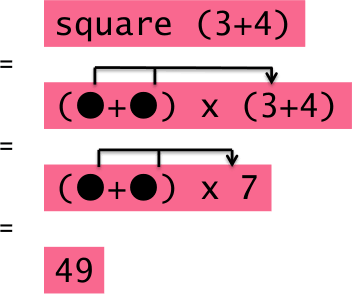
\includegraphics[width=0.25\linewidth]{mainmatter/pics/sharing}
\caption[Sharing + Outermost]{Sharing + Outermost}
\label{fig:sharing}
\end{figure}


  
  